\documentclass[conference]{IEEEtran}
\IEEEoverridecommandlockouts
\usepackage[T5,T1]{fontenc}
\usepackage[utf8]{inputenc}
% Macro to render Vietnamese sample phrases in Table VI without hijacking English labels
\newcommand{\vn}[1]{{\fontencoding{T5}\selectfont #1}}
\usepackage{cite}
\usepackage{amsmath,amssymb,amsfonts}
\usepackage{algorithmic}
\usepackage{graphicx}
\usepackage{textcomp}
\usepackage{xcolor}
\usepackage{booktabs}
\usepackage{multirow}
\usepackage{url}
\usepackage[hidelinks]{hyperref}

% STRICT ENFORCEMENT: Pure English IEEE Standard Labels (Overrides any language package or cache)
\makeatletter
\def\abstractname{Abstract}
\def\tablename{TABLE}
\def\figurename{Fig.}
\def\refname{REFERENCES}
\makeatother
\AtBeginDocument{
  \renewcommand{\abstractname}{Abstract}
  \renewcommand{\tablename}{TABLE}
  \renewcommand{\figurename}{Fig.}
  \renewcommand{\refname}{REFERENCES}
}

% Prevent isolated float pages: enforce tight packing with surrounding text
\renewcommand{\topfraction}{0.95}
\renewcommand{\bottomfraction}{0.95}
\renewcommand{\textfraction}{0.05}
\renewcommand{\floatpagefraction}{0.9}

\def\BibTeX{{\rm B\kern-.05em{\sc i\kern-.025em b}\kern-.08em
    T\kern-.1667em\lower.7ex\hbox{E}\kern-.125emX}}

\begin{document}

\title{An Empirical Comparison between Contextual Language Model PhoBERT and Classical TF-IDF for Vietnamese Student Feedback Sentiment Analysis\\
\thanks{All source code and experimental configurations are publicly available at \url{https://github.com/phanhuuy1107/my_paper_project} to facilitate full scientific reproducibility.}
}

\author{
\IEEEauthorblockN{Huu Y}
\IEEEauthorblockA{\textit{Faculty of Information Technology} \\
\textit{Undergraduate Research Program in AI/NLP}\\
Email: huuy.academic@gmail.com}
}

\maketitle

\begin{abstract}
Automated sentiment analysis of Vietnamese student feedback is essential for continuous quality assurance in higher education, yet it faces domain challenges including monosyllabic word boundary ambiguity, inverted comparative idioms, implicit negation, and severe class imbalance. In this paper, we establish a controlled empirical benchmark comparing a classical machine learning baseline (\textbf{TF-IDF with Multinomial Logistic Regression}) against a fine-tuned contextual language model (\textbf{PhoBERT-base}) across the official 16,175-sentence \textbf{UIT-VSFC} dataset.

Evaluations are conducted on an independent test set ($D_{\text{test}} = 3,166$ samples) across three random seeds ($42, 100, 2024$) under strict data leakage prevention protocols. Empirical findings demonstrate that PhoBERT-base achieves high stability and performance with \textbf{$82.95 \pm 0.69\%$ Macro-F1} and \textbf{$94.08 \pm 0.18\%$ Accuracy}, marking a \textbf{$+17.89$ pp} (percentage points) leap over the baseline ($65.06\%$). Crucially, bidirectional self-attention improves the minority Neutral class F1-score from $13.04\%$ to $59.64\%$ (\textbf{$+46.60$ pp}). An ablation study confirms that omitting syllable-level word segmentation incurs a substantial \textbf{$-5.46$ pp} Macro-F1 drop. Finally, a systematic comparative error taxonomy across five linguistic categories reveals that PhoBERT reduces total classification errors by \textbf{$48.3\%$} (from $354$ to $183$ mistakes), providing key empirical foundations for real-world educational feedback analysis systems.
\end{abstract}

\begin{IEEEkeywords}
Vietnamese NLP, Sentiment Analysis, PhoBERT, TF-IDF, Transformer Encoder, Macro-F1, Multi-seed, Ablation Study, Error Analysis, UIT-VSFC.
\end{IEEEkeywords}

\section{Introduction}
\subsection{Background and Motivation}
In modern higher education administration, collecting and analyzing student textual feedback plays a pivotal role in ensuring institutional teaching quality and curriculum improvement. However, manual review of tens of thousands of subjective feedback comments every academic semester imposes prohibitive human labor costs and fails to provide timely pedagogical interventions. Automating this workflow via Natural Language Processing (NLP) techniques is therefore an essential institutional objective.

\subsection{Formal Task Formulation}
We formulate the student feedback sentiment classification problem as a single-label supervised sequence mapping:
\begin{equation}
f: \mathcal{X} \to \mathcal{Y}
\end{equation}
where:
\begin{itemize}
    \item Input space $\mathcal{X}$: A sequence of Vietnamese lexical tokens $x_i = (w_1, w_2, \dots, w_n)$.
    \item Label space $\mathcal{Y}$: A discrete set of three sentiment categories:
    \begin{equation}
    \mathcal{Y} = \{0: \text{Negative}, 1: \text{Neutral}, 2: \text{Positive}\}
    \end{equation}
\end{itemize}
The optimization objective is to find an optimal parameter configuration $f^*$ that minimizes empirical cross-entropy loss over the unseen independent test distribution.

\subsection{Research Question}
This empirical investigation centers on addressing the following research question:
\begin{quote}
\textit{RQ: To what quantitative extent does the bidirectional contextual self-attention mechanism of PhoBERT outperform the traditional n-gram TF-IDF representation across individual imbalanced class distributions of UIT-VSFC, and what linguistic constructs continue to pose challenges for the model?}
\end{quote}

\subsection{Scientific Contributions}
This paper delivers three tangible contributions:
\begin{enumerate}
    \item \textbf{Controlled Multi-Seed Benchmark:} We establish an empirical evaluation on UIT-VSFC across three random seeds ($42, 100, 2024$), demonstrating the statistical stability and robustness of PhoBERT ($82.95 \pm 0.69\%$ Macro-F1, $+17.89\text{ pp}$ over baseline).
    \item \textbf{Mitigation of Class Imbalance \& Ablation Analysis:} We show that PhoBERT substantially improves classification on the minority Neutral class (raising F1 from $13.04\%$ to $59.64\%$, $+46.60\text{ pp}$), and empirically demonstrate that syllable-level word segmentation contributes $+5.46\text{ pp}$ to Macro-F1.
    \item \textbf{Systematic Comparative Error Taxonomy:} We classify and contrast the error distribution of both models across five linguistic obstacle categories without duplicate counting, proving that PhoBERT eliminates $48.3\%$ of baseline errors (reducing error count from $354$ to $183$).
\end{enumerate}

\section{Related Work}
Early research on Vietnamese sentiment analysis predominantly relied on hand-crafted lexical features combined with traditional classifiers such as Support Vector Machines (SVM) or Logistic Regression. In 2018, Nguyen et al.~\cite{vsfc2018} released the UIT-VSFC corpus comprising $16,175$ human-annotated student feedback sentences, which has since served as the standard benchmark in Vietnamese educational sentiment mining.

While the bag-of-words TF-IDF representation~\cite{manning2008introduction} offers computational efficiency, it inherently disregards word order and long-range contextual dependencies. The inception of the Transformer architecture~\cite{vaswani2017attention} and BERT~\cite{devlin2019bert} revolutionized NLP by establishing the pre-train-then-fine-tune paradigm. Building upon the RoBERTa architecture~\cite{liu2019roberta}, Nguyen and Nguyen~\cite{phobert2020} introduced PhoBERT, a monolingual model pre-trained on large-scale Vietnamese texts using word-level tokenization. However, comparative error breakdowns and multi-seed sensitivity analysis on educational feedback remain insufficiently explored.

\section{Methodology}
We evaluate two contrasting paradigms representing classical machine learning and modern deep contextual representations:

\subsection{Baseline Pipeline: TF-IDF + Logistic Regression}
Each input document $d$ is mapped to an n-gram feature vector $(1, 2)$ within a $10,000$-dimensional vocabulary:
\begin{equation}
\text{TF-IDF}(t, d, D) = \text{TF}(t, d) \times \left( \log \frac{|D|}{|\{d': t \in d'\}| + 1} + 1 \right)
\end{equation}
A linear classification layer computes the logit vector $z \in \mathbb{R}^3$, yielding class probabilities via the Softmax function:
\begin{equation}
P(y = c \mid x) = \frac{\exp(W_c^T x + b_c)}{\sum_{j=0}^2 \exp(W_j^T x + b_j)}
\end{equation}
Optimization is performed via the L-BFGS algorithm over multinomial cross-entropy loss with an $L_2$ regularization penalty using Scikit-learn~\cite{pedregosa2011scikit}.

\subsection{Proposed Model: PhoBERT-base Fine-Tuning}
We fine-tune the PhoBERT-base architecture~\cite{phobert2020,wolf2020transformers} comprising 12 Transformer Encoder layers, 12 attention heads, and a hidden state dimension of $d_{\text{model}} = 768$:
\begin{itemize}
    \item \textbf{Tokenization and Input Embeddings:} Raw text is segmented into compound words via \texttt{pyvi}~\cite{pyvi2016} and mapped to Byte-Pair Encoding (BPE) subwords prepended with the special token \texttt{[CLS]}:
    \begin{equation}
    X^{(0)} = E_{\text{token}} + E_{\text{pos}} \in \mathbb{R}^{N \times 768}
    \end{equation}
    \item \textbf{Multi-Head Self-Attention:}
    \begin{equation}
    \text{Attention}(Q, K, V) = \text{Softmax}\left(\frac{QK^T}{\sqrt{d_k}}\right)V
    \end{equation}
    \item \textbf{Classification Head:} The contextual pooled embedding $h_{[\text{CLS}]} \in \mathbb{R}^{768}$ from layer 12 is extracted and projected through a linear classification head:
    \begin{equation}
    z = h_{[\text{CLS}]} W_{\text{proj}} + b_{\text{proj}} \in \mathbb{R}^3
    \end{equation}
    The entire model is optimized end-to-end using AdamW~\cite{loshchilov2018decoupled} with decoupled weight decay.
\end{itemize}

\section{Experimental Setup}
\subsection{UIT-VSFC Dataset}
We adhere strictly to the official 7:1:2 train-validation-test split provided by the dataset creators~\cite{vsfc2018}, detailed in Table~\ref{tab:dataset}.

\begin{table}[!htbp]
\caption{Dataset Partition and Distribution in UIT-VSFC}
\label{tab:dataset}
\centering
\resizebox{\columnwidth}{!}{%
\begin{tabular}{lrrr}
\toprule
\textbf{Split} & \textbf{Sentences} & \textbf{Ratio (\%)} & \textbf{Role in Pipeline} \\
\midrule
Training ($D_{\text{train}}$) & $11,426$ & $70.6\%$ & Parameter optimization \\
Validation ($D_{\text{val}}$) & $1,583$ & $9.8\%$ & Checkpoint selection \\
Testing ($D_{\text{test}}$) & $3,166$ & $19.6\%$ & Unbiased final evaluation \\
\midrule
\textbf{Total} & \textbf{$16,175$} & \textbf{$100.0\%$} & Class balance: 43.7\% C0, 4.8\% C1, 51.5\% C2 \\
\bottomrule
\end{tabular}%
}
\end{table}

\subsection{Implementation and Hyperparameters}
Experiments were executed on an NVIDIA Tesla T4 GPU (Google Colab).
\begin{itemize}
    \item Batch size: 16 (training), 32 (evaluation).
    \item Maximum sequence length: 128 tokens; Epochs: 3.
    \item Optimizer: AdamW with peak learning rate $2 \times 10^{-5}$ and weight decay $0.01$.
    \item Leakage control: TF-IDF vocabulary and BPE tokenizers are fitted strictly on $D_{\text{train}}$.
\end{itemize}

\subsection{Evaluation Metrics}
Given the extreme class imbalance (the Neutral class accounts for only $4.8\%$ of instances), our primary metric is \textbf{Macro-F1}:
\begin{equation}
\text{Macro-F1} = \frac{1}{3} \sum_{c=0}^2 F_1^{(c)}, \quad F_1^{(c)} = \frac{2 P_c R_c}{P_c + R_c}
\end{equation}
Accuracy is reported alongside as an auxiliary global metric.

\section{Results and Discussion}
\subsection{Multi-Seed Robustness Benchmark}
Table~\ref{tab:overall_results} summarizes performance across three random seeds ($42, 100, 2024$) on the $3,166$-sentence test set.

\begin{table}[!htbp]
\caption{Performance on UIT-VSFC Test Set Across Random Seeds}
\label{tab:overall_results}
\centering
\resizebox{\columnwidth}{!}{%
\begin{tabular}{lccc}
\toprule
\textbf{Model Architecture} & \textbf{Accuracy (\%)} & \textbf{Macro-F1 (\%)} & \textbf{$\Delta$ Macro-F1} \\
\midrule
Baseline (TF-IDF + LR) & 88.82 (1 run) & 65.06 (1 run) & Reference \\
PhoBERT-base & \textbf{94.08 $\pm$ 0.18\%} & \textbf{82.95 $\pm$ 0.69\%} & \textbf{+17.89 pp} \\
\bottomrule
\end{tabular}%
}
\end{table}

The Baseline model produces deterministic results ($88.82\%$ Accuracy, $65.06\%$ Macro-F1). PhoBERT-base establishes an absolute gain of $+17.89\text{ pp}$ Macro-F1 (relative gain of $27.5\%$). The low variance ($\sigma = 0.69\text{ pp}$) across three distinct seeds confirms the algorithmic stability of fine-tuning.

\subsection{Per-Class Performance Breakdown}
Table~\ref{tab:per_class} delineates the class-wise performance discrepancies on Seed 42.

\begin{table}[!t]
\caption{Detailed Per-Class Performance Comparison on Seed 42}
\label{tab:per_class}
\centering
\resizebox{\columnwidth}{!}{%
\begin{tabular}{lcccccc}
\toprule
\multirow{2}{*}{\textbf{Sentiment Class}} & \multicolumn{3}{c}{\textbf{Baseline (TF-IDF + LR)}} & \multicolumn{3}{c}{\textbf{PhoBERT-base}} \\
\cmidrule(lr){2-4} \cmidrule(lr){5-7}
& Precision & Recall & F1-score & Precision & Recall & F1-score \\
\midrule
0: Negative & 0.8506 & 0.9659 & 0.9046 & \textbf{0.9467} & \textbf{0.9702} & \textbf{0.9583} \\
1: Neutral  & 0.7059 & 0.0719 & 0.1304 & \textbf{0.7593} & \textbf{0.4910} & \textbf{0.5964} \\
2: Positive & 0.9290 & 0.9050 & 0.9169 & \textbf{0.9504} & \textbf{0.9648} & \textbf{0.9576} \\
\midrule
\textbf{Macro Average} & 0.8285 & 0.6476 & 0.6506 & \textbf{0.8855} & \textbf{0.8087} & \textbf{0.8374} \\
\bottomrule
\end{tabular}%
}
\end{table}

\noindent The most critical improvement occurs in the minority Neutral class: PhoBERT lifts the F1-score from $13.04\%$ to $59.64\%$ ($+46.60\text{ pp}$), with Recall expanding nearly sevenfold (from $7.19\%$ to $49.10\%$). This demonstrates that self-attention effectively captures nuanced, objective statements that lack explicit polarizing keywords.

\subsection{Ablation Study: Word Segmentation}
Table~\ref{tab:ablation} isolates the impact of Vietnamese compound word segmentation (\texttt{pyvi}):

\begin{table}[!htbp]
\caption{Ablation Study on Vietnamese Word Segmentation (Seed 42, 1 run)}
\label{tab:ablation}
\centering
\resizebox{\columnwidth}{!}{%
\begin{tabular}{lccc}
\toprule
\textbf{Model Configuration} & \textbf{Accuracy} & \textbf{Macro-F1} & \textbf{$\Delta$ F1} \\
\midrule
PhoBERT Full (With \texttt{pyvi}) & \textbf{94.22\%} & \textbf{83.74\%} & Reference \\
PhoBERT Unsegmented (No \texttt{pyvi}) & 91.66\% & 78.28\% & \textbf{-5.46 pp} \\
\bottomrule
\end{tabular}%
}
\end{table}

Omitting word segmentation fragments multi-syllable terms into sub-optimal BPE tokens, incurring a sharp $-5.46\text{ pp}$ drop in Macro-F1. This empirically confirms that syllable-level compound segmentation is indispensable for Vietnamese Transformer encoders.

\section{Comparative Error Analysis}
Table~\ref{tab:error_comparison} presents a mutually exclusive categorization of incorrect predictions between Baseline ($354$ errors, consistent with $88.82\%$ accuracy) and PhoBERT ($183$ errors, consistent with $94.22\%$ accuracy) across five core linguistic challenge categories on the test set ($N = 3,166$).

\begin{table}[!htbp]
\caption{Mutually Exclusive Error Distribution Across 5 Categories}
\label{tab:error_comparison}
\centering
\resizebox{\columnwidth}{!}{%
\begin{tabular}{lccc}
\toprule
\textbf{Linguistic Error Category} & \textbf{Baseline} & \textbf{PhoBERT} & \textbf{Reduction} \\
\midrule
1. Neutral $\leftrightarrow$ Polarized Ambiguity & 236 & 145 & -91 (-38.6\%) \\
2. Inverted Comparative Idioms with Negation & 4 & 1 & -3 (-75.0\%) \\
3. Double Negation \& Long-range Contrast & 19 & 11 & -8 (-42.1\%) \\
4. Annotation Noise & 2 & 1 & -1 (-50.0\%) \\
5. Slang, Teencode, and Abbreviations & 93 & 25 & -68 (-73.1\%) \\
\midrule
\textbf{Total Errors (on 3,166 test samples)} & \textbf{354} & \textbf{183} & \textbf{-171 (-48.3\%)} \\
\bottomrule
\end{tabular}%
}
\end{table}

PhoBERT reduces total classification errors by $48.3\%$ (eliminating $171$ false predictions). Subword BPE representations resolve $73.1\%$ of errors arising from non-standard student slang and abbreviations. Fig.~\ref{fig:confusion_matrix} displays the normalized confusion matrix of PhoBERT on the test set. Table~\ref{tab:error_cases} presents qualitative case studies of representative errors.

\begin{figure}[!htbp]
\centering
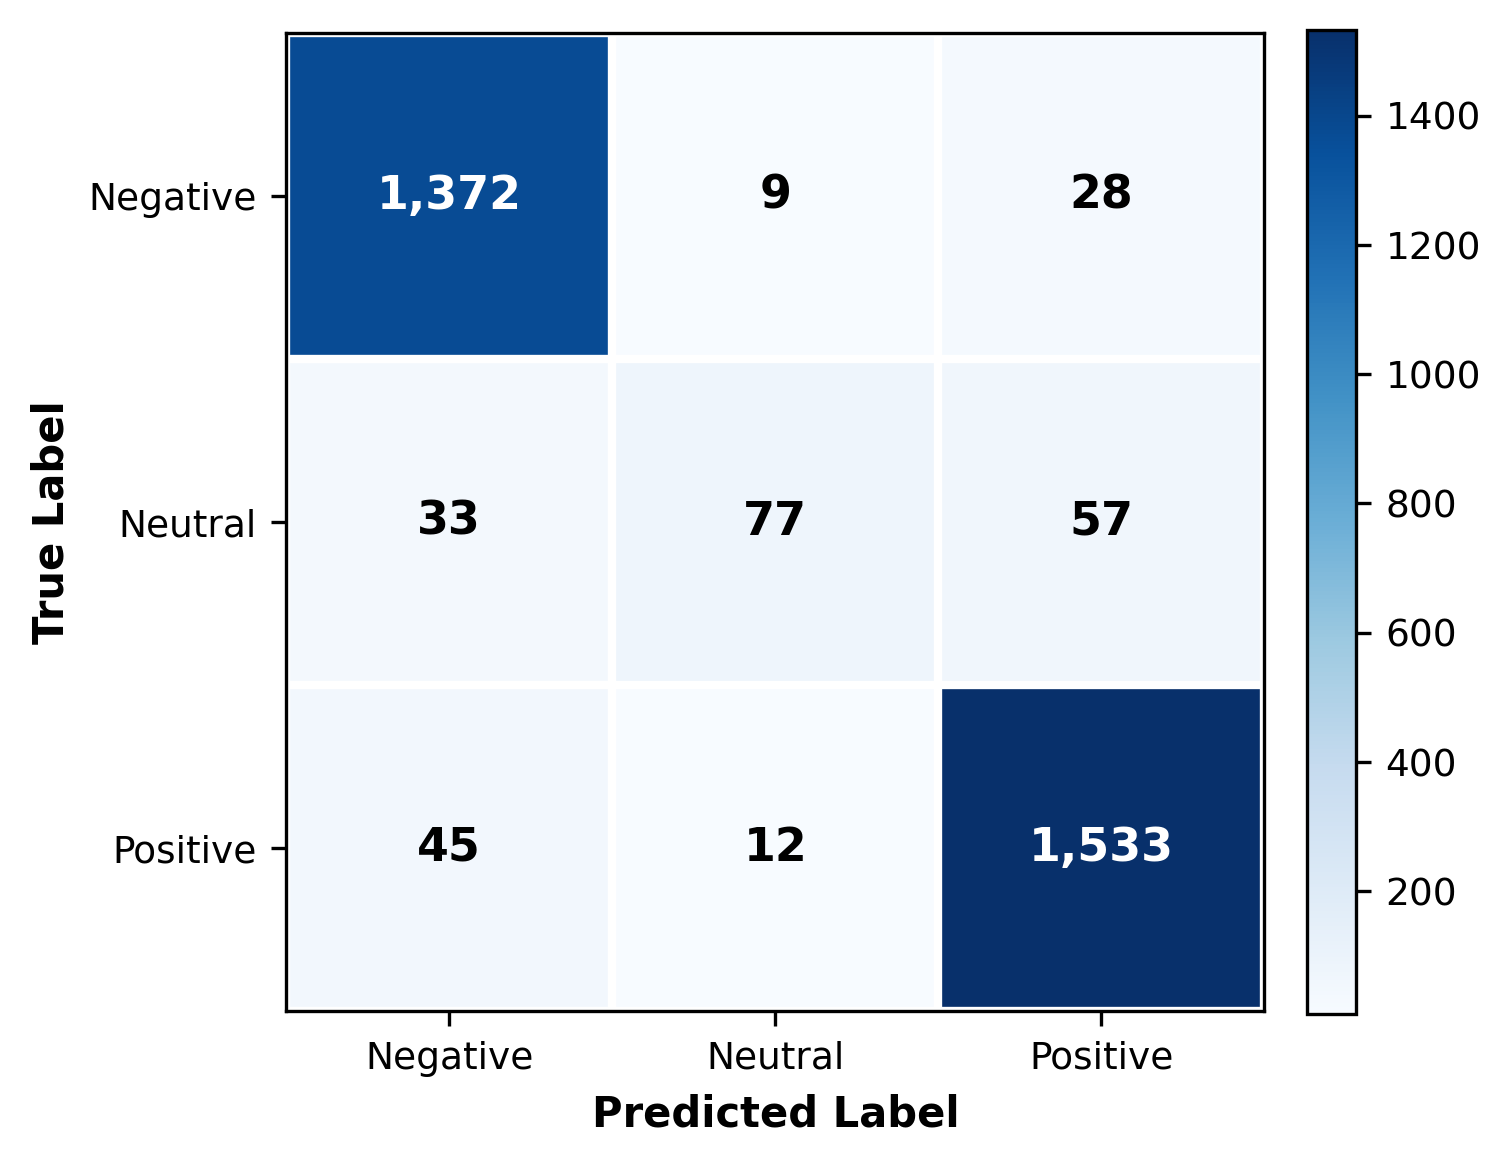
\includegraphics[width=0.82\columnwidth]{confusion_matrix.png}
\caption{Confusion Matrix of PhoBERT-base on the UIT-VSFC Test Set ($N=3,166$, Seed 42).}
\label{fig:confusion_matrix}
\end{figure}

\begin{table*}[!t]
\caption{Qualitative Analysis of Representative Error Cases on UIT-VSFC Test Set}
\label{tab:error_cases}
\centering
\resizebox{\textwidth}{!}{%
\begin{tabular}{clccl}
\toprule
\textbf{ID} & \textbf{Student Feedback Sentence (English Translation \& Vietnamese Source)} & \textbf{Gold} & \textbf{Predicted} & \textbf{Underlying Linguistic Mechanism} \\
\midrule
\#12 & ``If instructor's macbook is second, no laptop is first.'' & Positive & Negative & Inverted comparative idiom with surface negation marker (``no/none''). \\
     & \textit{\footnotesize [Vietnamese: \vn{trong trường macbook thầy số hai thì không có máy nào số một .}]} & & & Self-attention over-attends to negation token, overpowering idiomatic praise. \\
\midrule
\#45 & ``Mostly just theory and exercises.'' & Positive & Negative & Annotation noise; the restrictive marker (``only/merely'') carries negative critique, \\
     & \textit{\footnotesize [Vietnamese: \vn{phần lớn chỉ là lý thuyết và bài tập .}]} & & & yet ground truth was annotated as positive in the benchmark corpus. \\
\midrule
\#35 & ``This course helped us understand fundamental concepts.'' & Neutral & Positive & Latent positive sentiment in educational phrasing (``helped us understand'') shifts hidden \\
     & \textit{\footnotesize [Vietnamese: \vn{môn học này giúp chúng em hiểu ra những vấn đề cơ bản .}]} & & & representation towards the Positive class boundary. \\
\midrule
\#53 & ``That way we will have better orientation and focus...'' & Neutral & Positive & Strongly polarized comparative keyword (``better'') overpowers the overall neutral \\
     & \textit{\footnotesize [Vietnamese: \vn{như vậy tụi em sẽ định hướng tốt hơn và tập trung...}]} & & & consultative tone of the statement. \\
\midrule
\#6  & ``Calculate competition points for groups.'' & Positive & Neutral & Objective declarative administrative statement erroneously annotated as Positive \\
     & \textit{\footnotesize [Vietnamese: \vn{tính điểm thi đua các nhóm .}]} & & & in ground truth; PhoBERT correctly infers neutral semantic tone. \\
\bottomrule
\end{tabular}%
}
\end{table*}

\section{Ethics Statement and Limitations}
\subsection{Ethics Statement}
This research uses the publicly released UIT-VSFC benchmark~\cite{vsfc2018}, which was curated for academic research purposes. Feedback comments were anonymized prior to public release to remove student and instructor personal identifiers. The sentiment classification models developed herein are designed strictly for institutional pedagogical evaluation and educational quality enhancement, and should not be employed for punitive assessments or surveillance of academic personnel.

\subsection{Limitations}
We explicitly acknowledge several methodological limitations of the current study:
\begin{itemize}
    \item \textbf{Single Dataset Scope:} All empirical evaluations were conducted exclusively on the UIT-VSFC benchmark. Cross-domain generalizability across other Vietnamese sentiment datasets (e.g., e-commerce reviews or social media posts) remains to be assessed.
    \item \textbf{Single Classical Baseline:} We compared PhoBERT against a single traditional baseline (TF-IDF + Logistic Regression). While TF-IDF represents standard Bag-of-Words practice, future work should incorporate multilingual Transformer baselines such as mBERT or XLM-RoBERTa~\cite{conneau2020unsupervised}.
    \item \textbf{Absence of Statistical Significance Testing:} Model comparisons were evaluated via mean and standard deviation across three seeds. Formal paired hypothesis testing (e.g., McNemar's test on per-instance predictions) was not conducted.
    \item \textbf{Constrained Compute Infrastructure and Single-Seed Ablation:} Due to resource limits of free-tier GPU instances (Tesla T4), the ablation study was executed on a single seed (Seed 42) rather than multi-seed trials, and hyperparameter tuning was restricted to standard recommended learning rates.
    \item \textbf{Minority Class Performance:} Despite marked gains, the Neutral class Recall ($49.10\%$) indicates that nearly half of neutral feedback comments remain misclassified due to severe $4.8\%$ label scarcity.
\end{itemize}

\section{Conclusion and Future Work}
This paper presented a controlled empirical comparison contrasting PhoBERT-base with a classical TF-IDF baseline on the UIT-VSFC benchmark. Across three random seeds, PhoBERT demonstrated high stability, delivering a $+17.89\text{ pp}$ leap in Macro-F1 and decreasing total error cases by $48.3\%$ ($354 \to 183$). In future work, we plan to incorporate loss functions designed for class imbalance such as Focal Loss~\cite{lin2017focal} to address remaining minority boundaries, perform formal significance tests, and explore model quantization for efficient edge deployment.

\bibliographystyle{IEEEtran}
\bibliography{references}

\end{document}
